\documentclass[letter,10pt]{article}
\usepackage[utf8]{inputenc}

\title{Influence maximization }
\author{Víctor Emiliano Cruz Hernández}

%\usepackage[spanish]{babel}
\usepackage{listings}
\usepackage{graphicx} 
\usepackage{amsthm}
\usepackage{amsmath}
\usepackage{mathtools}
\usepackage{ amssymb }
\usepackage{algorithm2e}
\usepackage{tikz}


%% This is needed if you want to add comments in
%% your algorithm with \Comment
\SetKwComment{Comment}{/* }{ */}
\SetKwRepeat{Do}{do}{while}
\RestyleAlgo{ruled}

\DeclarePairedDelimiter\ceil{\lceil}{\rceil}
\DeclarePairedDelimiter\floor{\lfloor}{\rfloor}

\theoremstyle{definition}
\newtheorem{definition}{Definition}[section]

\newtheorem{theorem}{Theorem}

\begin{document}

\maketitle

% This document is an example of BibTeX using in bibliography management. Three items are cited: \textit{The \LaTeX\ Companion} book \cite{latexcompanion}, the Einstein journal paper \cite{einstein}, and the Donald Knuth's website \cite{knuthwebsite}. The \LaTeX\ related items are \cite{latexcompanion,knuthwebsite}. 

\section{Introduction}

Finding the most influential people is a NP-Hard problem. Authors have formalized the problem as: 
\begin{center}
    \textit{Given a weighted graph in which nodes are people and edge weights represent the influence of the people on each other it is desired to find $k$ starting nodes that their activation leads to maximum propagation based on a chosen influence maximization model}.
\end{center}

Assume we have data on a graph which estimates which individuals influence on others. We would like to market a new product that we hope will be adopted by a large fraction of the network by initially targeting a few "influential" members of the network and giving them free samples of the product, hoping we can maximize the number of people influenced by this individual. The problem aims to find a number of people that are able to maximize the spread of influence through a target social network.

\subsection{Influence Maximization model}.

In this section we will explain how in our model we say a person is influenced by it's peers. There are two most prevalent diffusion models in computer science; the independent cascade and linear threshold model, both have different properties that concern our influence maximization problem. We will not take further detail on which one we will use, as we just lead the following idea:

Given a $threshold$ value $\theta$ and our di-graph $G=(V,E)$ where $v_i \in V$ is a person and $W=\{u_0, \dots , u_k\} \subset V$ is the set of people such that for $j\in \{0,\dots k\}$, $(u_j, v_i) \in E$. We say that $v_i$ is influenced iff:
\begin{align*}
    \sum_{u\in W}w( (u,v_i) ) \geq \theta
\end{align*}

Where $w((u,v_i))$ is the weigth of the $(u, v_i)$ edge.


Instead of pursuing a "cascade of influence" were influencers can spread their influence further it's own neighbors. We restrict their influence in the scope of their immediate neighbors in $G$. 

We can take for example the following digraph with $\theta = 0.5$. In this example, we should be able to find  for $k=2$ the set $\{v_1, v_4\}$ as the set of $k$ influencers who reach the most influenced nodes $\{v_2, v_3, v_5\}$. 


\begin{center}
\tikzset{every picture/.style={line width=0.75pt}} %set default line width to 0.75pt        

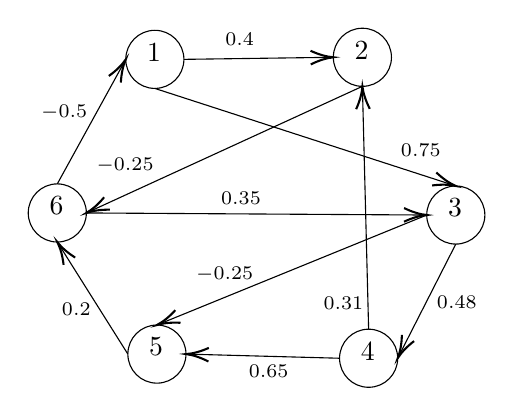
\begin{tikzpicture}[x=0.75pt,y=0.75pt,yscale=-1,xscale=1]
%uncomment if require: \path (0,199); %set diagram left start at 0, and has height of 199

%Shape: Circle [id:dp7559594892259189] 
\draw   (251,27) .. controls (251,19.27) and (257.27,13) .. (265,13) .. controls (272.73,13) and (279,19.27) .. (279,27) .. controls (279,34.73) and (272.73,41) .. (265,41) .. controls (257.27,41) and (251,34.73) .. (251,27) -- cycle ;
%Shape: Circle [id:dp04563686399300515] 
\draw   (351,26) .. controls (351,18.27) and (357.27,12) .. (365,12) .. controls (372.73,12) and (379,18.27) .. (379,26) .. controls (379,33.73) and (372.73,40) .. (365,40) .. controls (357.27,40) and (351,33.73) .. (351,26) -- cycle ;
%Shape: Circle [id:dp7827953676750938] 
\draw   (396,102) .. controls (396,94.27) and (402.27,88) .. (410,88) .. controls (417.73,88) and (424,94.27) .. (424,102) .. controls (424,109.73) and (417.73,116) .. (410,116) .. controls (402.27,116) and (396,109.73) .. (396,102) -- cycle ;
%Shape: Circle [id:dp7079532928811787] 
\draw   (354,171) .. controls (354,163.27) and (360.27,157) .. (368,157) .. controls (375.73,157) and (382,163.27) .. (382,171) .. controls (382,178.73) and (375.73,185) .. (368,185) .. controls (360.27,185) and (354,178.73) .. (354,171) -- cycle ;
%Shape: Circle [id:dp5540537345240124] 
\draw   (252,169) .. controls (252,161.27) and (258.27,155) .. (266,155) .. controls (273.73,155) and (280,161.27) .. (280,169) .. controls (280,176.73) and (273.73,183) .. (266,183) .. controls (258.27,183) and (252,176.73) .. (252,169) -- cycle ;
%Shape: Circle [id:dp05253436056064231] 
\draw   (204,101) .. controls (204,93.27) and (210.27,87) .. (218,87) .. controls (225.73,87) and (232,93.27) .. (232,101) .. controls (232,108.73) and (225.73,115) .. (218,115) .. controls (210.27,115) and (204,108.73) .. (204,101) -- cycle ;
%Straight Lines [id:da16879741834635498] 
\draw    (218,87) -- (250.04,28.75) ;
\draw [shift={(251,27)}, rotate = 118.81] [color={rgb, 255:red, 0; green, 0; blue, 0 }  ][line width=0.75]    (10.93,-3.29) .. controls (6.95,-1.4) and (3.31,-0.3) .. (0,0) .. controls (3.31,0.3) and (6.95,1.4) .. (10.93,3.29)   ;
%Straight Lines [id:da6740287828167513] 
\draw    (279,27) -- (349,26.03) ;
\draw [shift={(351,26)}, rotate = 179.2] [color={rgb, 255:red, 0; green, 0; blue, 0 }  ][line width=0.75]    (10.93,-3.29) .. controls (6.95,-1.4) and (3.31,-0.3) .. (0,0) .. controls (3.31,0.3) and (6.95,1.4) .. (10.93,3.29)   ;
%Straight Lines [id:da9395970972630745] 
\draw    (365,40) -- (233.82,100.17) ;
\draw [shift={(232,101)}, rotate = 335.36] [color={rgb, 255:red, 0; green, 0; blue, 0 }  ][line width=0.75]    (10.93,-3.29) .. controls (6.95,-1.4) and (3.31,-0.3) .. (0,0) .. controls (3.31,0.3) and (6.95,1.4) .. (10.93,3.29)   ;
%Straight Lines [id:da9452224478879836] 
\draw    (265,41) -- (408.1,87.38) ;
\draw [shift={(410,88)}, rotate = 197.96] [color={rgb, 255:red, 0; green, 0; blue, 0 }  ][line width=0.75]    (10.93,-3.29) .. controls (6.95,-1.4) and (3.31,-0.3) .. (0,0) .. controls (3.31,0.3) and (6.95,1.4) .. (10.93,3.29)   ;
%Straight Lines [id:da002878871948137407] 
\draw    (368,157) -- (365.05,42) ;
\draw [shift={(365,40)}, rotate = 88.53] [color={rgb, 255:red, 0; green, 0; blue, 0 }  ][line width=0.75]    (10.93,-3.29) .. controls (6.95,-1.4) and (3.31,-0.3) .. (0,0) .. controls (3.31,0.3) and (6.95,1.4) .. (10.93,3.29)   ;
%Straight Lines [id:da9488630562987759] 
\draw    (410,116) -- (382.91,169.22) ;
\draw [shift={(382,171)}, rotate = 296.98] [color={rgb, 255:red, 0; green, 0; blue, 0 }  ][line width=0.75]    (10.93,-3.29) .. controls (6.95,-1.4) and (3.31,-0.3) .. (0,0) .. controls (3.31,0.3) and (6.95,1.4) .. (10.93,3.29)   ;
%Straight Lines [id:da9544783714587981] 
\draw    (354,171) -- (282,169.05) ;
\draw [shift={(280,169)}, rotate = 1.55] [color={rgb, 255:red, 0; green, 0; blue, 0 }  ][line width=0.75]    (10.93,-3.29) .. controls (6.95,-1.4) and (3.31,-0.3) .. (0,0) .. controls (3.31,0.3) and (6.95,1.4) .. (10.93,3.29)   ;
%Straight Lines [id:da198745934825584] 
\draw    (252,169) -- (219.07,116.69) ;
\draw [shift={(218,115)}, rotate = 57.8] [color={rgb, 255:red, 0; green, 0; blue, 0 }  ][line width=0.75]    (10.93,-3.29) .. controls (6.95,-1.4) and (3.31,-0.3) .. (0,0) .. controls (3.31,0.3) and (6.95,1.4) .. (10.93,3.29)   ;
%Straight Lines [id:da4383193154517051] 
\draw    (232,101) -- (394,101.99) ;
\draw [shift={(396,102)}, rotate = 180.35] [color={rgb, 255:red, 0; green, 0; blue, 0 }  ][line width=0.75]    (10.93,-3.29) .. controls (6.95,-1.4) and (3.31,-0.3) .. (0,0) .. controls (3.31,0.3) and (6.95,1.4) .. (10.93,3.29)   ;
%Straight Lines [id:da7285408756013072] 
\draw    (396,102) -- (267.85,154.24) ;
\draw [shift={(266,155)}, rotate = 337.82] [color={rgb, 255:red, 0; green, 0; blue, 0 }  ][line width=0.75]    (10.93,-3.29) .. controls (6.95,-1.4) and (3.31,-0.3) .. (0,0) .. controls (3.31,0.3) and (6.95,1.4) .. (10.93,3.29)   ;

% Text Node
\draw (260,18) node [anchor=north west][inner sep=0.75pt]   [align=left] {1};
% Text Node
\draw (360,17) node [anchor=north west][inner sep=0.75pt]   [align=left] {2};
% Text Node
\draw (405,93) node [anchor=north west][inner sep=0.75pt]   [align=left] {3};
% Text Node
\draw (363,162) node [anchor=north west][inner sep=0.75pt]   [align=left] {4};
% Text Node
\draw (261,160) node [anchor=north west][inner sep=0.75pt]   [align=left] {5};
% Text Node
\draw (213,92) node [anchor=north west][inner sep=0.75pt]   [align=left] {6};
% Text Node
\draw (209,47.73) node [anchor=north west][inner sep=0.75pt]  [font=\scriptsize]  {$-0.5$};
% Text Node
\draw (297.67,13.07) node [anchor=north west][inner sep=0.75pt]  [font=\scriptsize]  {$0.4$};
% Text Node
\draw (235.67,73.07) node [anchor=north west][inner sep=0.75pt]  [font=\scriptsize]  {$-0.25$};
% Text Node
\draw (382.33,66.4) node [anchor=north west][inner sep=0.75pt]  [font=\scriptsize]  {$0.75$};
% Text Node
\draw (345,140.4) node [anchor=north west][inner sep=0.75pt]  [font=\scriptsize]  {$0.31$};
% Text Node
\draw (399.67,139.73) node [anchor=north west][inner sep=0.75pt]  [font=\scriptsize]  {$0.48$};
% Text Node
\draw (309,173.07) node [anchor=north west][inner sep=0.75pt]  [font=\scriptsize]  {$0.65$};
% Text Node
\draw (219,143.07) node [anchor=north west][inner sep=0.75pt]  [font=\scriptsize]  {$0.2$};
% Text Node
\draw (295.67,89.73) node [anchor=north west][inner sep=0.75pt]  [font=\scriptsize]  {$0.35$};
% Text Node
\draw (283.67,125.73) node [anchor=north west][inner sep=0.75pt]  [font=\scriptsize]  {$-0.25$};


\end{tikzpicture}

\end{center}

Notice that $v_2$ is influenced. For $W=\{v_1, v_4\}$ we see that:
\begin{align*}
    \sum_{u\in W}w( (u,v_2) ) = w((v_1, v_2) + w((v_4, v_2)) = 0.4 + 0.31  = 0.71\geq \theta = 0.5
\end{align*}

\section{Heuristic}
We use Ant Colony Optimization (ACO) as C.Salavati and A.Abdollahpouri presented in their paperwork \cite{main_file}.
\subsection{Neighborhood}

Let $D = (V,E)$ our initial relation graph. We use the following definitions for building the neighborhood graph $N_D$.

\begin{definition}[$similarity(u,v)$] Let $u,v\in V$ where $outN(u), outN(v)$ are the out-neighbors of $u,v$ respectively.  And $outN2(u)$ as the set of all neighbors of the neighbors of $u$:

\[
outN2(u) =
\bigcup_{w\in outN(u)} outN(w)
\]

We define the similarity of $u,v$, $similarity(u,v)$ as:

\[
similarity(u,v) = 
     \begin{cases}
       1 & u\in outN(v)\\
       \alpha \frac{|outN(u) \cap outN(v)|}{|outN(u) \cup outN(v)|}+
       \beta \frac{|outN2(u) \cap outN2(v)|}{|outN2(u) \cup outN2(v)|}
       & otherwise\\
       
     \end{cases}
\]
\end{definition}

Note that this relation is not symetric since we have a digraph and $\beta$ and $\alpha$ have to satisfy $\alpha +\beta = 1$ so we can tune the impact of direct users over second hand users. 

\begin{definition}[Neighborhood Graph: $N_D$] Given a relational wighted digraph $D=(V,E)$ We define our neighborhood graph $N_D=(V_{ND}, E_{ND}, W_{ND}, S_{ND})$ where:
\begin{itemize}
    \item $V_{ND} = V$
    \item $E_{ND} = \binom {V_{ND}}2$
    \item $W_{ND} = E$
    \item $S_{ND} = \{ similarity(u,v) | u,v\in V_{ND}\}$
    \item $P_{ND} = \{ pheromone(u,v) | u,v\in V_{ND}\}$
\end{itemize}

\end{definition}

We define our graph as a complete digraph where the edges between are calculated with the original weight in $D$ and the similarity between the two nodes and the pheromone value. Initialy for all $u,v\in V_{ND}$, $pheromone(u,v) = \tau_0$, we set an initial pheromone value to all edges in $E_{ND}$.


\subsection{State transition rule}

We use the neighborhood graph $N_D$ to select the $k$ influencers that maximize the influence in the original graph $D$. Initially we select a random node in $N_D$. 

Let $T=[v_0,\dots,v_i] $ be the current selected nodes and $v_i$ the last one selected. Then we have to select the next node $v_j$ with a \textit{state transition rule }. It is a greedy rule defined by:
\begin{itemize}
    \item The pheromone value of $(v_i, v_j)$: $phermomone(v_i, v_j) \in P_{ND}$.
    \item The \textit{profit value rule}: $profitValue(T \cup \{v_j\})$.
    \item The \textit{mutual similarity rule}: $S(T \cup \{ v_j \})$.
\end{itemize}
We proceed to define such rules:

\begin{definition}[Profit value rule: $profitValue(T,v_j)$] Let $T$ be the set of current selected nodes and $v_j$ the next node to select. We define the \textit{profit value rule} of $T$ and $v_j$ as:
\[ 
    profitValue(T) = r \sum_{u\in V_{ND}} influenced(T , u) - ck 
\]
where 
\[
influenced(T,u) = 
     \begin{cases}
       1 & \sum_{r\in T}w( (r,u) ) \geq \theta\\
       0 & otherwise\\
     \end{cases}
\]
where:
\begin{itemize}
    \item $r$ is a parameter which is the revenue from buying a product.
    \item $c$ is the cost of selecting a node as influence node.
    \item $k$ is the size of our desire influence node set.
\end{itemize}
\end{definition}
The \textit{profit value rule} allows us to calculate how many nodes are influenced by a given set of nodes $T$.

\begin{definition}[Mutual similarity rule: $S(T)$] We define the \textit{mutual similarity rule} as :
\[
    S(T) = \sum_{u\in T}\sum_{v\in T} similarity(u,v)
\]
    
\end{definition}
This is the amount of similarity that a set of nodes $T$ has between each pair of themselves.

Finally we can define the \textit{state transition rule} as follow:

\begin{definition}[State transition rule: $greedTransition(T=(v_0, \dots, v_i))$ ] 
Let $T$ be the current set of selected nodes, we select the next node greedly by:
    \[
        greedTransition(T =[v_0, \dots, v_i] ) = max_{v_j \in V_{ND}-T} \big \{ edgeValue( T, v_j)\big \}
    \]
    where:
\begin{align*}
        edgeValue(T=[v_0,\dots,v_i], v_j) ]= &pheromone(v_i, v_j)^\eta * \\
        &profitValue(T\cup \{v_j\})^\psi *\\
        &S(T\cup \{v_j\})^\gamma
    \end{align*}
    where $\eta$, $\psi$, $\gamma$ are a parameters used to control the importance of pheromone trail versus heuristic information.
\end{definition}

\subsection{Fitness}

After an ant has finished constructing its path, we evaluate the suitability og each path scrolled with a \textit{fitness function}. It is a combination of the \textit{profit value} and \textit{mutual similarity}.

\begin{definition}[Fitness function: $fitness( T )$] Given a path $T$ we evaluate the path with te \textit{fitness function } as:
\[
    fitness(T) = profitValue(T)^\psi * \Big (\frac{1}{S(T)} \Big )^\gamma
\]
    
\end{definition}

\subsection{Pheromone update}

After an ant has completed it's path we update the pheromome of each edge in $P_{ND}$ as follows:
Let $T$ be the path build by the ant.
\[
    pheromone(v_i,v_j)_t = (1-\rho) pheromone(v_i,v_j)_{t-1} + fitness(T)
\]
where $t-1$ is the inmediate past iteration of iteration $t$.
    
\newpage


\section{Implementation}

\subsection{Generation of the graph}
We used a real dataset for testing our system. The Extended Epinions collection, collected by Paolo Massa. The datasets we use can be found in \texttt{epinions/}. It contains two files \texttt{rating\_relation.csv} where we can found users that qualify other user's job and \texttt{user\_rating.csv} where we have the relation between two users as the trust/distrustment a user have on another. 

\subsubsection{rating\_relation.csv}
This file represent the ratings a user has given to other user. A posible line in the file can be like this: \texttt{317856,234885,5}. We can read the line as the edge $(317856,234885)$ where user $317856$ rated $234885$ with a $5$.

In the database, a user can rate another user in a natural number between 1 and 5. The dataset is not consistent as it has some ratings over 5, for the generation of the graph we take the following scale over the rating:

\begin{center}
    \begin{tabular} { | m{5em} | m{1cm}|} 
      \hline
       Scale setting & Rating \\ 
      \hline
       1 & 5 \\ 
       0.75 & 4 \\ 
       0.25 & 3 \\ 
       -1 & 2 \\ 
       -1 & 1 \\ 
      \hline
    \end{tabular}
\end{center}

Note that a user $u$ can rate other user $v$ multiple times. For convenience, we denote as $A_{uv}[i]$ as the $i$-th rate user $u$ gives to $v$.

\subsubsection{user\_rating.csv}

This file contains the relation of trust/distrustment one user have over another. A line in this file looks like \texttt{361404,81580625796,-1} meaning that user $361404$ distrust user $81580625796$. If we change it to \texttt{361404,81580625796,1} now it means user $361404$ trust user $81580625796$.

 With the previous information we can generate the relation sub-graph with the weights representing both datasets. Given a pair of users $u,v$ we define the weigth of the edge $(u,v)$ as:
 \[
    w(u,v) = 
    \begin{cases}
       1 &  \textit{if $v$ trust $u$} \\
       -1 &  \textit{if $v$ distrust $u$} \\
       \frac{1-e^{-x}}{1+e^{-x}} & \textit{if user v rates u} \\
       0 & otherwise 
     \end{cases}
 \]
where:
\[
    x = f(u,v) = \sum_{i\in A_{uv}} A_{uv}[i]
\]
$f(u,v)$ will be positive if the sum of all ratings that $u$ has given to $v$ is positive and negative if the sum is negative. This way the edges of the graph we generate have weights between $[-1,1]$. 
\subsubsection{Generation of the sub-graph}

With those datasets, given a seed $s$ we can generate a random graph of $n$ nodes, for example, we can create a graph of \texttt{500} nodes with seed \texttt{10} in the file \texttt{./graph500S10.csv}.

\begin{center}
    \texttt{\$ cargo run --release graph 500 10 ./graph500S10.csv  }
\end{center}

We show the last 10 lines of the file:\\
%\begin{center}
    \texttt{200396,369121,1}\\
    \texttt{255170,200396,0.46211717}\\
    \texttt{500873,2147483647,1}\\
    \texttt{2147483647,217293,1}\\
    \texttt{255170,525533,0.12435301}\\
    \texttt{530381,483904,-1}\\
    \texttt{253067,2147483647,1}\\
    \texttt{341013,329733,0.90514827}\\
    \texttt{315491,262868,0.46211717}\\
    \texttt{322084,2147483647,0.9969976}\\
%s\end{center}

We can take the first line \texttt{200396,369121,1} wich represent the directed edge $(200396,369121)$ of weight $1$.

With any of the graph generated this way we can excecute the second part of the system searching the desire $k$ influencers in the graph.

\subsection{Path finding in a graph}
Given a graph generated previously and a seed $s$ we can find the $k$ influencers in the graph as follows:
\begin{center}
    \texttt{\$ cargo run --release expr ./graph500S10.csv 20 5000 }
\end{center}

This way we search for the set of $k=20$ nodes  5,000 times and show the path $T$ when it finishes with a given seed. We show some ot the previous execution's results:

\texttt{FITNESS: 2.891806, SEED: 41}\\
\texttt{SOLUTION: [Node { id: 489989 }, Node { id: 561193 }, Node { id: 282884 }, Node { id: 2147483647 }, Node { id: 538395 }, Node { id: 610716 }, Node { id: 514960 }, Node { id: 548930 }, Node { id: 374388 }, Node { id: 211440 }, Node { id: 536828 }, Node { id: 605439 }, Node { id: 500873 }, Node { id: 437453 }, Node { id: 245729 }, Node { id: 440719 }, Node { id: 540403 }, Node { id: 223319 }, Node { id: 569385 }, Node { id: 406551 }]}
\\\\
\texttt{FITNESS: 2.652228, SEED: 42}\\
\texttt{SOLUTION: [Node { id: 523809 }, Node { id: 450802 }, Node { id: 304628 }, Node { id: 538395 }, Node { id: 221034 }, Node { id: 408214 }, Node { id: 326696 }, Node { id: 768511876 }, Node { id: 211440 }, Node { id: 497699 }, Node { id: 257170 }, Node { id: 488144 }, Node { id: 2147483647 }, Node { id: 390490 }, Node { id: 494303 }, Node { id: 507426 }, Node { id: 368476 }, Node { id: 499006 }, Node { id: 557444 }, Node { id: 518224 }]}

A lower fitness function represent better results

\section{Results}
This problem is widely studied and used. It can take several approaches such as first selecting the influence maximization model. The way we present this problem and a solution is simple enough to compare results with brute force results yet complicated enough it is unfeasible to scale this comparison in larger graphs. \\

There is a unfinished approach in representing visually the results, this could help in the experimentation stage. A complete tuning of the system requires this step, furthermore complete this project adequately.
\medskip

\bibliographystyle{unsrt}%Used BibTeX style is unsrt
\nocite{*}
\bibliography{sample}


\end{document}
